\documentclass[14pt]{extbook}
\usepackage{multicol, enumerate, enumitem, hyperref, color, soul, setspace, parskip, fancyhdr} %General Packages
\usepackage{amssymb, amsthm, amsmath, latexsym, units, mathtools} %Math Packages
\everymath{\displaystyle} %All math in Display Style
% Packages with additional options
\usepackage[headsep=0.5cm,headheight=12pt, left=1 in,right= 1 in,top= 1 in,bottom= 1 in]{geometry}
\usepackage[usenames,dvipsnames]{xcolor}
\usepackage{dashrule}  % Package to use the command below to create lines between items
\newcommand{\litem}[1]{\item#1\hspace*{-1cm}\rule{\textwidth}{0.4pt}}
\pagestyle{fancy}
\lhead{Makeup Progress Quiz 2}
\chead{}
\rhead{Version A}
\lfoot{2790-1423}
\cfoot{}
\rfoot{Summer C 2021}
\begin{document}

\begin{enumerate}
\litem{
Choose the graph of the equation below.\[ f(x) = \frac{1}{(x - 2)^2} - 3 \]\begin{enumerate}[label=\Alph*.]
\begin{multicols}{2}\item 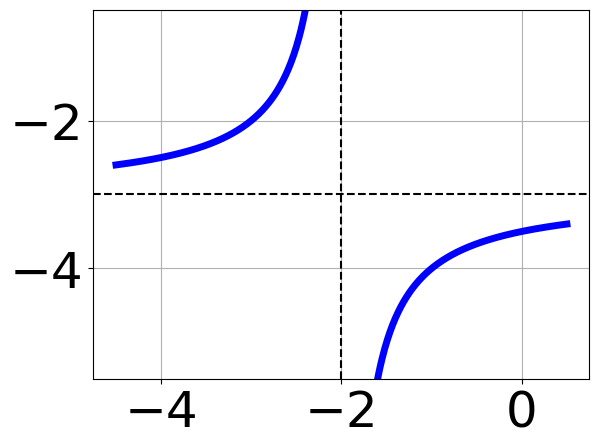
\includegraphics[width = 0.3\textwidth]{../Figures/rationalEquationToGraphAA.png}\item 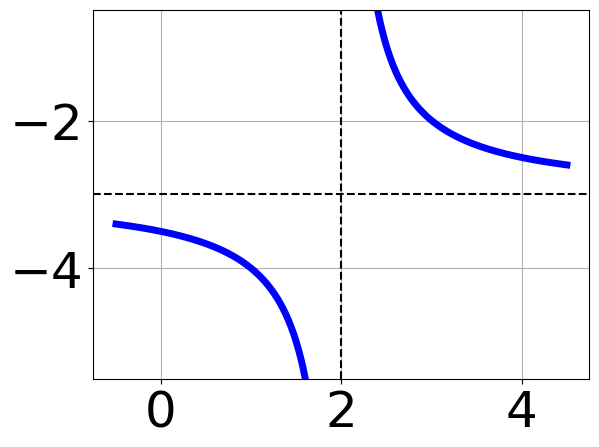
\includegraphics[width = 0.3\textwidth]{../Figures/rationalEquationToGraphBA.png}\item 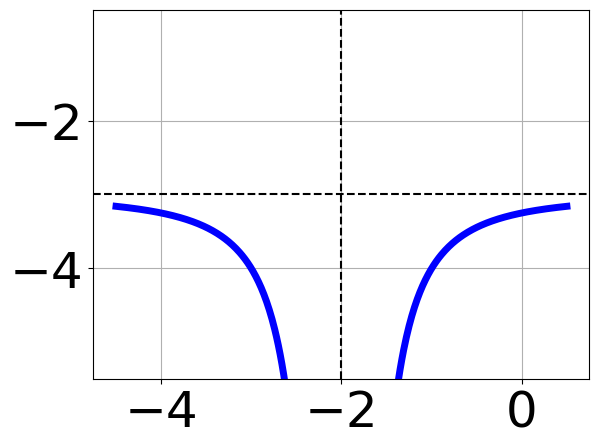
\includegraphics[width = 0.3\textwidth]{../Figures/rationalEquationToGraphCA.png}\item 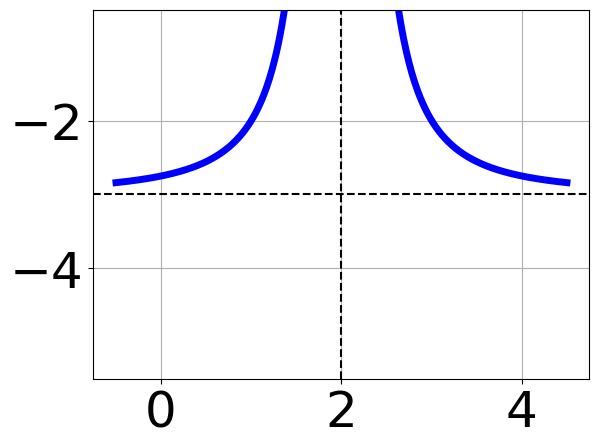
\includegraphics[width = 0.3\textwidth]{../Figures/rationalEquationToGraphDA.png}\end{multicols}\item None of the above.
\end{enumerate} }
\litem{
Solve the rational equation below. Then, choose the interval(s) that the solution(s) belongs to.\[ \frac{8}{5x -5} + 5 = \frac{-2}{40x -40} \]\begin{enumerate}[label=\Alph*.]
\item \( x \in [-1.35,-1.3] \)
\item \( x_1 \in [0.58, 0.63] \text{ and } x_2 \in [-0.33,2.67] \)
\item \( x \in [0.67,2.67] \)
\item \( \text{All solutions lead to invalid or complex values in the equation.} \)
\item \( x_1 \in [-1.35, -1.3] \text{ and } x_2 \in [-0.33,2.67] \)

\end{enumerate} }
\litem{
Choose the graph of the equation below.\[ f(x) = \frac{-1}{(x - 2)^2} - 1 \]\begin{enumerate}[label=\Alph*.]
\begin{multicols}{2}\item 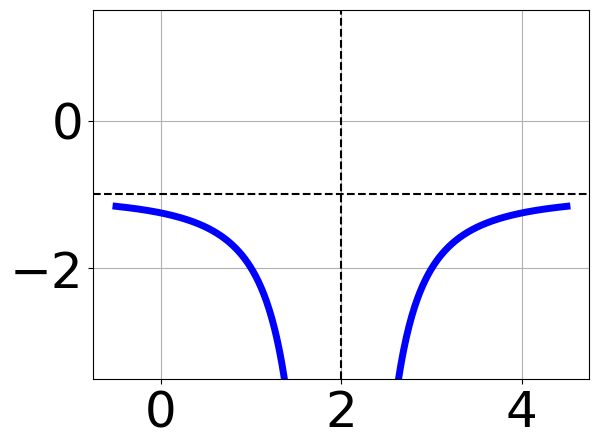
\includegraphics[width = 0.3\textwidth]{../Figures/rationalEquationToGraphCopyAA.png}\item 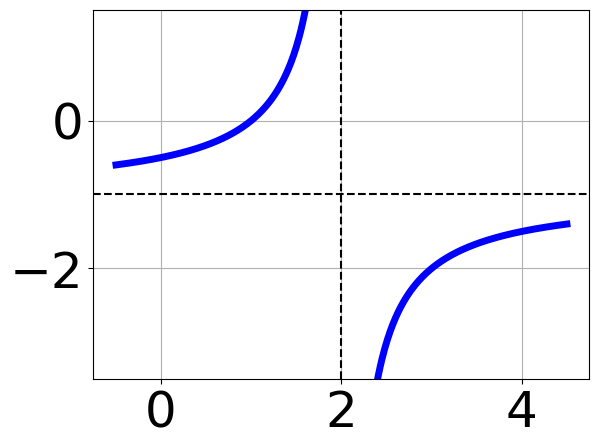
\includegraphics[width = 0.3\textwidth]{../Figures/rationalEquationToGraphCopyBA.png}\item 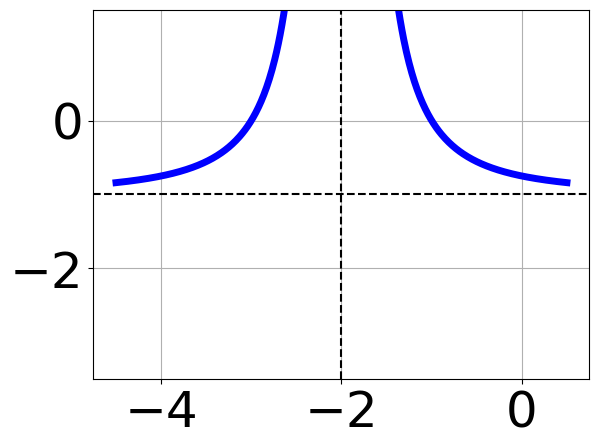
\includegraphics[width = 0.3\textwidth]{../Figures/rationalEquationToGraphCopyCA.png}\item 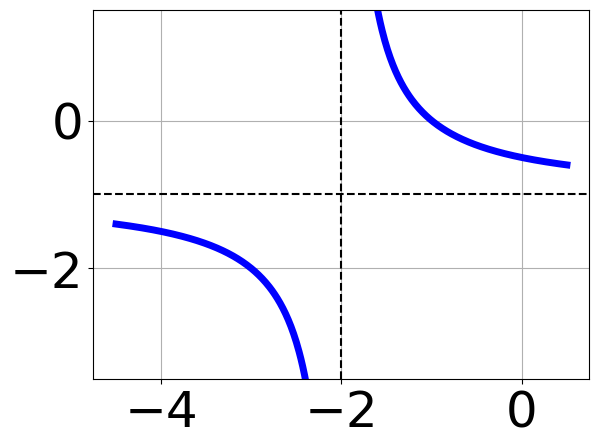
\includegraphics[width = 0.3\textwidth]{../Figures/rationalEquationToGraphCopyDA.png}\end{multicols}\item None of the above.
\end{enumerate} }
\litem{
Solve the rational equation below. Then, choose the interval(s) that the solution(s) belongs to.\[ \frac{50}{20x + 90} + 1 = \frac{50}{20x + 90} \]\begin{enumerate}[label=\Alph*.]
\item \( x \in [-5.5,-2.5] \)
\item \( x \in [3.5,6.5] \)
\item \( \text{All solutions lead to invalid or complex values in the equation.} \)
\item \( x_1 \in [-5.5, -3.5] \text{ and } x_2 \in [-5.5,-2.5] \)
\item \( x_1 \in [-5.5, -3.5] \text{ and } x_2 \in [3.5,6.5] \)

\end{enumerate} }
\litem{
Determine the domain of the function below.\[ f(x) = \frac{3}{20x^{2} -45 x + 25} \]\begin{enumerate}[label=\Alph*.]
\item \( \text{All Real numbers except } x = a, \text{ where } a \in [-0.9, 1.2] \)
\item \( \text{All Real numbers.} \)
\item \( \text{All Real numbers except } x = a \text{ and } x = b, \text{ where } a \in [-0.9, 1.2] \text{ and } b \in [1.1, 1.6] \)
\item \( \text{All Real numbers except } x = a, \text{ where } a \in [19.7, 21.6] \)
\item \( \text{All Real numbers except } x = a \text{ and } x = b, \text{ where } a \in [19.7, 21.6] \text{ and } b \in [23.9, 26.9] \)

\end{enumerate} }
\litem{
Choose the equation of the function graphed below.
\begin{center}
    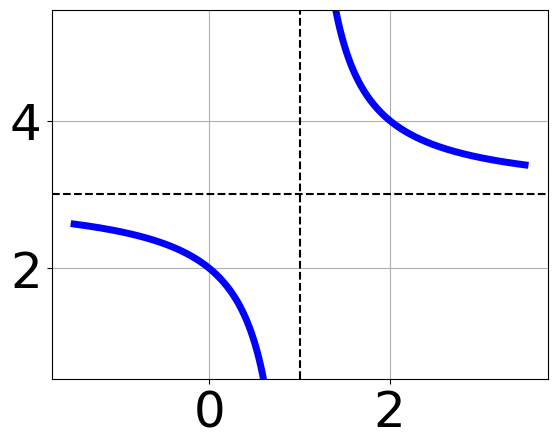
\includegraphics[width=0.5\textwidth]{../Figures/rationalGraphToEquationA.png}
\end{center}
\begin{enumerate}[label=\Alph*.]
\item \( f(x) = \frac{1}{x - 1} + 3 \)
\item \( f(x) = \frac{1}{(x - 1)^2} + 3 \)
\item \( f(x) = \frac{-1}{x + 1} + 3 \)
\item \( f(x) = \frac{-1}{(x + 1)^2} + 3 \)
\item \( \text{None of the above} \)

\end{enumerate} }
\litem{
Determine the domain of the function below.\[ f(x) = \frac{5}{30x^{2} +12 x -18} \]\begin{enumerate}[label=\Alph*.]
\item \( \text{All Real numbers.} \)
\item \( \text{All Real numbers except } x = a, \text{ where } a \in [-38, -35] \)
\item \( \text{All Real numbers except } x = a \text{ and } x = b, \text{ where } a \in [-38, -35] \text{ and } b \in [15, 17] \)
\item \( \text{All Real numbers except } x = a, \text{ where } a \in [-3, 0] \)
\item \( \text{All Real numbers except } x = a \text{ and } x = b, \text{ where } a \in [-3, 0] \text{ and } b \in [0.6, 1.6] \)

\end{enumerate} }
\litem{
Choose the equation of the function graphed below.
\begin{center}
    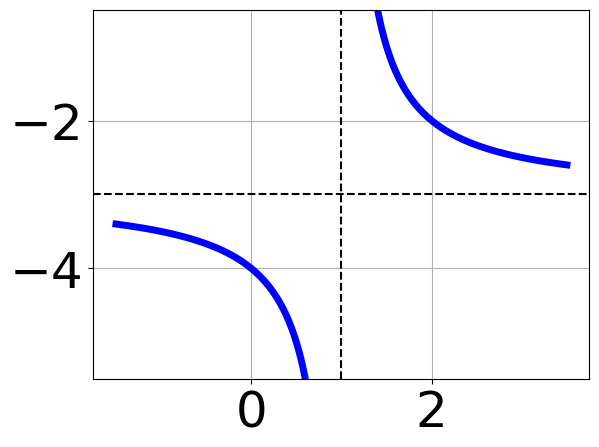
\includegraphics[width=0.5\textwidth]{../Figures/rationalGraphToEquationCopyA.png}
\end{center}
\begin{enumerate}[label=\Alph*.]
\item \( f(x) = \frac{1}{(x - 1)^2} - 3 \)
\item \( f(x) = \frac{-1}{(x + 1)^2} - 3 \)
\item \( f(x) = \frac{1}{x - 1} - 3 \)
\item \( f(x) = \frac{-1}{x + 1} - 3 \)
\item \( \text{None of the above} \)

\end{enumerate} }
\litem{
Solve the rational equation below. Then, choose the interval(s) that the solution(s) belongs to.\[ \frac{-5x}{-6x + 3} + \frac{-7x^{2}}{24x^{2} -36 x + 12} = \frac{5}{-4x + 4} \]\begin{enumerate}[label=\Alph*.]
\item \( x_1 \in [0.64, 0.78] \text{ and } x_2 \in [-2.37,0.11] \)
\item \( x \in [0.86,1.04] \)
\item \( x_1 \in [0.64, 0.78] \text{ and } x_2 \in [-0.58,1.58] \)
\item \( \text{All solutions lead to invalid or complex values in the equation.} \)
\item \( x \in [-1.77,-1.5] \)

\end{enumerate} }
\litem{
Solve the rational equation below. Then, choose the interval(s) that the solution(s) belongs to.\[ \frac{5x}{3x -6} + \frac{-2x^{2}}{-12x^{2} +12 x + 24} = \frac{-4}{-4x -4} \]\begin{enumerate}[label=\Alph*.]
\item \( x_1 \in [1.77, 3.6] \text{ and } x_2 \in [-1.17,-0.95] \)
\item \( x \in [-2.56,0.83] \)
\item \( x \in [1.77,3.6] \)
\item \( x_1 \in [-0.3, 0.93] \text{ and } x_2 \in [-2.17,-1.08] \)
\item \( \text{All solutions lead to invalid or complex values in the equation.} \)

\end{enumerate} }
\end{enumerate}

\end{document}